\chapter{Inleiding}
De hedendaagse meest gebruikte database management systemen (DBMS's) zijn de relationele DBMS's of NoSQL systemen \cite{dbengine-ranking}. In deze thesis beschrijft een testmethode om beide systemen te kunnen vergelijken op basis van consistentie en beschikbaarheid, welke daarna toegepast wordt als voorbeeld op MongoDB, HBase en Pgpool-II (een uitbreiding van PostgreSQL). 

Het RDBM is er gekomen onder invloed van het artikel van E. Codd over het relationele model in 1969 \cite{codd1970relational}. Het sleutelconcept van het relationele model is dat de data georganiseerd is in tabellen, gekoppeld door sletuels (constraints). Dit concept leidt tot een vermindering van de redundante data. 
Voorbeelden van populaire relationele DBMS's (RDBMS's) zijn Oracle, MySQL en PostgreSQL. 

De NoSQL databases zijn een nieuwe generatie van systemen, de NoSQL beweging is gestart in 2000 en staat voor '\textit{Not only SQL}'. Deze systemen zijn er gekomen als op de globalisering van de computer systemen. Met een geografische spreiding van de verschillende datacentra konden de RDBMS niet om?. Dit leidde tot de nood voor meer flexibele databases, een lagere complexiteit, hogere doorvoer van data, horizontale schaalbaarheid en het draaien op commodity hardware. NoSQL DBMS proberen hieraan te voldoen met voorbeelden als Google BigTable, Amazon Dynamo, HBase, MongoDB, ... \cite{Strauch.NoSQL} 

In de volgende sectie zullen beide systemen in meer detail aanbod komen, waarna de huidige staat voor het kwantitatief vergelijken van de systemen aan bod. Tenslotte zullen de doelstellingen en de bijdragen van de thesis toegelicht worden. 

\section{Relationele en NoSQL DBMS's} 
Op dit moment zijn de meest gebruikte DBMS's de relationele en NoSQL systemen, maar wat dit net inhoudt en wat de verschillen tussen beiden zijn, zal in deze sectie in meer detail aanbod komen. Eerst zullen het relationele DBMS besproken worden, gevolgd door NoSQL een een korte bespreking van de grootste verschillen. 

\subsection{Relationele database}
Een RDBMS is een DBMS gebaseerd op relationele model voor het structuren van de database.

Het relationele model is vertrekt van theoretische wiskundige principes als set-theorie en eerste-orde predicaten logica. Het model organiseert de data in tabellen en relaties tussen de tabellen. De tabel heeft kolommen die verschillende velden voorstellen waarbij elke rij een collectie van gerelateerde datawaardes is. De relaties tussen de verschillende tabellen toont hoe deze bij elkaar horen. Een belangrijke eigenschap is dat de tabellen en relaties genormaliseerd worden, hiermee wordt redundante informatie verwijderd. Dit zorgt voor een hogere data integriteit en een vermindering in data anomalieën die kunnen optreden bij een update.\cite{Elmasri:2010:FDS:1855347} \\
De normalisatie kan geïllustreerd worden met het korte voorbeeld van figuur \ref{fig:Relationeel-Model-Normalisatie}: de professor voor een vak zal bij elke student hetzelfde zijn, het veranderen van een professor voor een vak zou in het eerste geval een update van alle ingeschreven studenten inhouden, in het tweede geval is dit maar de aanpassing van een enkel record, hetzelfde geldt voor de student. \\
Interactie met de RDBMS gebeurt op basis van SQL (Structured Query Language), een taal gebaseerd op de relationele logica. SQL geeft uitgebreide query mogelijkheden aan de gebruiker van de software.   
\begin{figure}[ht!]
\centering
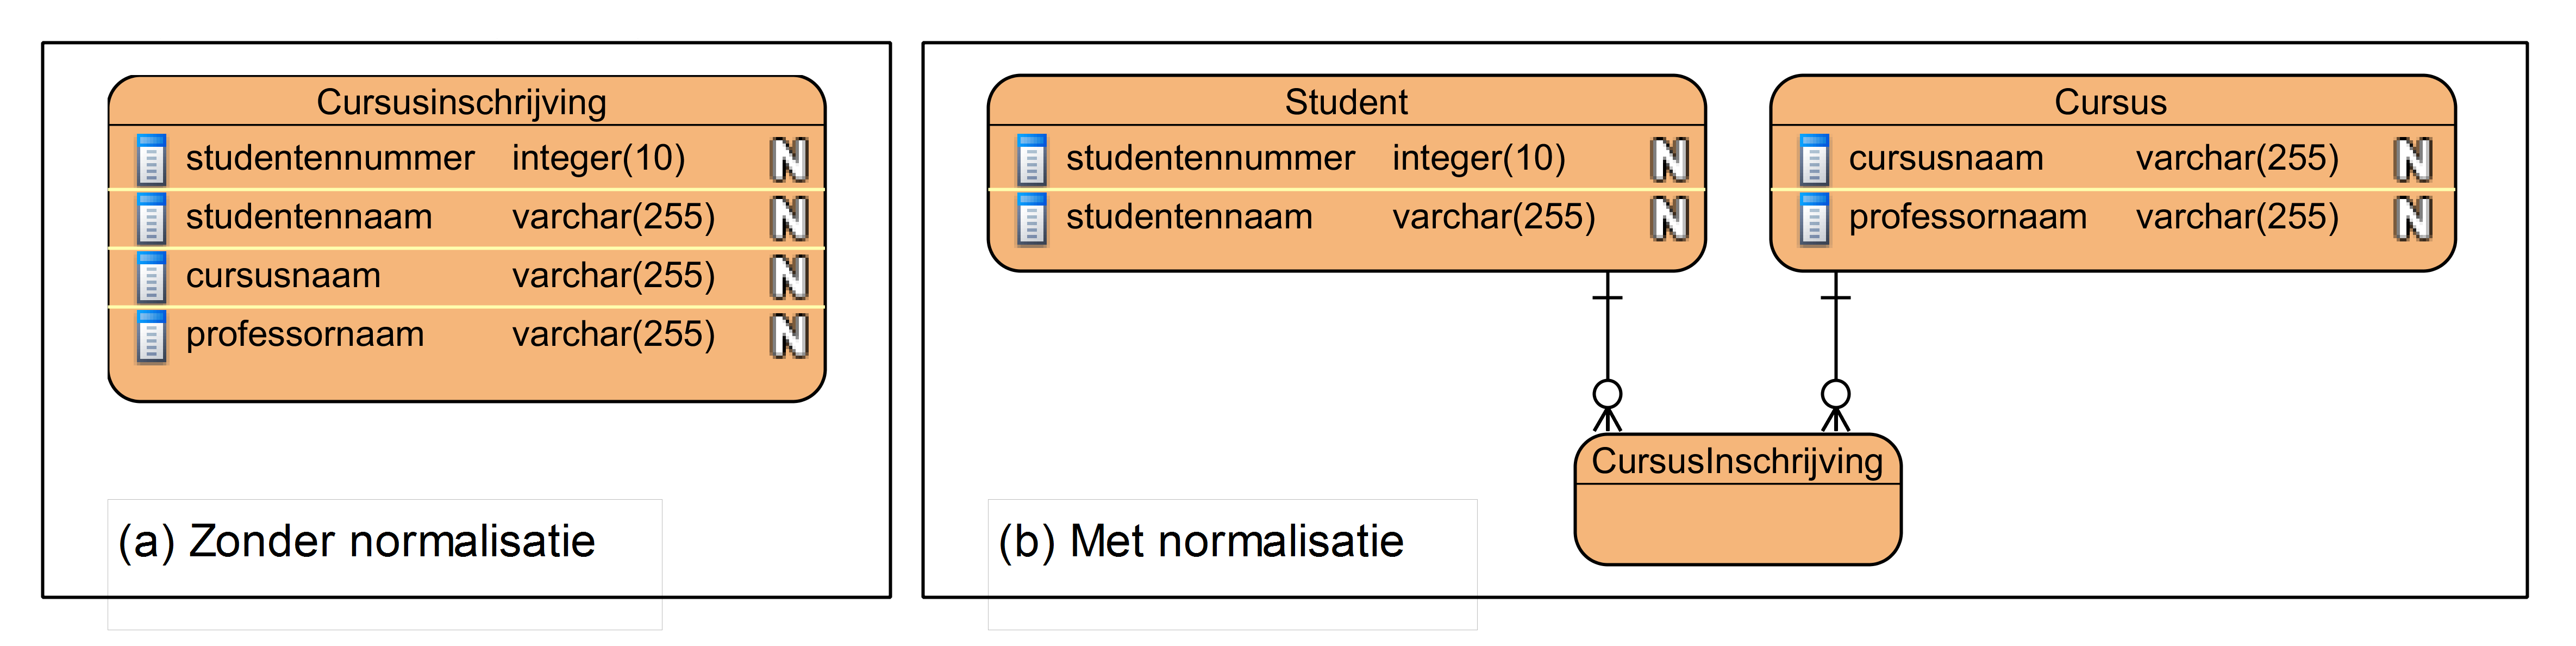
\includegraphics[width=\linewidth]{img/Relationeel-Model-Normalisatie.png}
\caption[Relationeel datamodel (a) zonder en (b) met normalisatie]{Relationeel datamodel (a) zonder en (b) met normalisatie}
\label{fig:Relationeel-Model-Normalisatie}
\end{figure}

Een belangrijk concept in een relationele database is ACID, welk voor betrouwbare en robuuste transacties zorgt

\paragraph{Atomair (\underline{A}tomicity)} Een database transactie moet oftewel volledig uitgevoerd worden oftewel heeft geen enkele bewerking plaatsgevonden. 

\paragraph{Consistent (\underline{C}onsistency)} Een transactie behoudt consistentie als de volledige uitvoering van de transactie de database van één consistente staat naar een andere brengt. Een consistente staat is een staat die ervoor zorgt dat waardes van een instantie consistent zijn met de andere waarden in dezelfde staat. Een voorbeeld is het overschrijven van \euro{50} van persoon A naar B, op het einde moet de totale som nog steeds gelijk zijn, A \euro{50} minder en B \euro{50} meer. Een inconsistente staat zou zijn dat enkel A \euro{50} minder heeft, maar B nog steeds evenveel. 

\paragraph{Geïsoleerd (\underline{I}solation)} Een transactie moet uitgevoerd worden alsof ze volledig voor of na andere transacties heeft plaatsgevonden. 

\paragraph{Duurzaam (\underline{D}urability)} Een voltooide transactie kan later niet ongedaan gemaakt worden.

Deze verschillende concepten bieden de garanties welke de gebruiker kan gebruiken voor zijn systeem. Daartegen over staat wel dat dit de complexiteit van de RDBMS groeit, ook indien dit voor bepaalde toepassingen misschien niet nodig is.

\subsection{NoSQL database\cite{Strauch.NoSQL}}\label{sec:eventualconsistency}
NoSQL DBMS zijn ontstaan door een groei en globalisering van de computersystemen en de bijhorende databases. Een RDBMS is gebouwd met een 'one size fits all'-gedachte, maar deze systemen hiermee complexiteit die voor bepaalde toepassingen niet nodig is. NoSQL systemen bestaan in verschillende variëteiten, elk met hun eigen eigenschappen en toepassingsgebied om zo de complexiteit te verminderen. Tussen deze verschillen is er een rode draad te vinden vergeleken met een RDBMS:
\begin{itemize}
	\item \textbf{Lagere complexiteit}: NoSQL systemen bieden minder opties en garanties dan de RDBMS, bepaalde applicaties hebben enkel nood aan een deel van de garanties. Bijvoorbeeld in een sociale netwerk moet een post niet onmiddellijk beschikbaar zijn voor al de vrienden van een persoon, maar dit mag even duren.
	\item \textbf{Hogere doorvoer}: Talrijke NoSQL systemen bieden een hogere doorvoer van data aan wat in veel gevallen een gevolg is van de lagere complexiteit of door de hulp van andere bewerkingen zoals MapReduce \cite{dean2008mapreduce}.
	
	\item \textbf{Horizontale schaalbaarheid en werkend op commodity hardware}: Waar grote RDBMS's werken met dure high-end systemen, was het bedoeling van NoSQL databases ondersteuning te bieden aan een veelvoud van geclusterde eenvoudige machines (commodity hardware). \\
	Horizontale schaalbaarheid staat voor het toevoegen extra machines aan een systeem voor extra resources, in tegenstelling tot verticale schaalbaarheid waar een krachtiger machine wordt gebruikt voor de opschaling. De horizontale opschaling wordt tot uitvoering gebracht door de data van een enkele database of tabel te verspreiden over verschillende machines die elk maar voor een deel van de data verantwoordelijk zijn en moeten opslaan.\\
	NoSQL systemen combineren deze twee elementen en bieden hierdoor een schaalbaar systeem aan met basis componenten.
	\item \textbf{Datamodel dichter bij objecten}: De meeste NoSQL systemen zijn zodanig ontworpen dat deze de vertaling van objecten naar opslag eenvoudiger maken t.o.v. RDBMS's. RDBMS zijn ontworpen voor het ontstaan van object georiënteerde programmeertalen en heeft de nood aan de vertaling van een object naar de databasestructuur. Bij het ontwerp van NoSQL werd er hiermee onmiddellijk rekening gehouden.  
\end{itemize}  \noindent
Deze verschillende argumenten leiden vervolgens tot BASE, een tegenreactie op ACID. \noindent 
\begin{itemize}
 \item Basis beschikbaarheid (\textbf{B}asically \textbf{Availability}): het DBMS biedt lees- en schrijfacties aan bij het falen van één of meerdere falende instanties. De ondersteuning is afhankelijk van systeem tot systeem samen met de configuratie
 \item \textbf{S}oft State: De data moet op een bepaald moment niet volledig consistent zijn. 
 \item Eventuele consistentie (\textbf{E}ventual Consistency): De database zal na enige tijd in een consistente status uitkomen, het is mogelijk dat oudere data tijdelijk leesbaar is. Eventuele consistentie kan op zijn beurt opnieuw onderverdeeld worden in 4 categorieën \cite[slide 16]{lipcon2009design}:
 	\begin{itemize}
 		\item \textit{Read your own writes} consistentie: Ongeachte van de server waarop een gebruiker leest, zal hij zijn schrijfactie onmiddellijk correct lezen. 
 		\item \textit{Session} consistentie: De gebruiker zal zijn schrijfactie onmiddellijk kunnen lezen binnen dezelfde sessie, een sessie is hierdoor meestal gelimiteerd tot een enkele database server. 
 		\item \textit{Casual} consistentie: Als een gebruiker versie X leest en vervolgens versie Y schrijft, zal elke gebruiker die versie Y leest ook versie X lezen.
 		\item \textit{Monotonic Read} consistentie: Dit levert monotone tijdsgaranties dat een gebruiker enkel recentere data versies in de toekomst zal lezen. 
 	\end{itemize}
\end{itemize}
De BASE eigenschappen kunnen gekoppeld worden aan de CAP theorie van Erik Brewer\cite{Brewer:2000:TRD:343477.343502}. CAP zegt dat een gedistribueerd systeem maar twee van de 3 CAP elementen kan ondersteunen: consistentie, beschikbaarheid en partitie tolerantie. De beschikbaarheid betekent dat bij het falen van een instantie er nog steeds schrijfbewerkingen mogelijk zijn. Bij partitie tolerantie kan het systeem overweg met het opgesplitst zijn van instantie door een niet werkende netwerk verbinding. De definitie van consistentie is hier anders als bij ACID: bij CAP is er sprake van consistentie als het DBMS zich gedraagt alsof er maar een enkel kopie van de data is.

\subsubsection{Classificatie van NoSQL systemen}
Er zijn vele NoSQL systemen ontworpen gedurende de laatste jaren, elk met hun eigen variëteit, functionaliteit en populariteit. Er bestaan verschillende manieren om de systemen te classificeren, maar één van de meest gebruikte doet dit op basis de data modellering. Een korte vergelijking op basis van deze bevindt zich in tabel \ref{table:selectie-classificatie}.  

\begin{table}[!h]
	\resizebox{\textwidth}{!} {
		\begin{tabular}{l l l l l l}
			\textbf{Soort} & \textbf{Performantie} & \textbf{Schaalbaarheid} & 			\textbf{Flexibiliteit} & \textbf{Complexiteit} & \textbf{Functionaliteit} \\ \hline
			Column & hoog & hoog & gematigd & laag & minimaal \\
			Document & hoog & variabel(hoog) & hoog & laag & variabel (laag) \\
			Graph & variabel & variabel & hoog & hoog & graph theory \\
			Key-Value & hoog & hoog & hoog & geen & variabel (geen) \\
		\end{tabular}
	}
	\caption{Classificatie en categorisatie van NoSQL DBMS's door Scofield en Popescu. \cite{categorizatie-sco10} \cite{categorizatie-pop10b} }
	\label{table:selectie-classificatie}
\end{table} 

\paragraph{Column Model}In een column-gebaseerd systeem wordt de data opgeslagen per kolom in plaats van de traditionele manier, per rij. Deze aanpak werd in eerste instantie gedaan voor analyse van business intelligentie. Het systeem is geïnspireerd door de paper van Google’s Bigtable \cite{chang2008bigtable}. \cite{Strauch.NoSQL}

\paragraph{Graph Model} In een grafen model, wordt de data voorgesteld en opslagen volgens de grafen theorie: knopen, lijnen en eigenschappen op de knopen en lijnen. \cite{bollacker2008freebase}.   

\paragraph{Key-Value Model} Key-Value systemen hebben een heel eenvoudig data model, data kan opgeslagen, opgevraagd en verwijderd worden op basis van een key. De informatie die in de database zit, is de waarde voor die key. \\
Met dit eenvoudig model en functionaliteit die weinig complexiteit introduceren, kan er gestreefd worden naar een hoge performantie, schaalbaarheid en flexibiliteit. \cite{Strauch.NoSQL}

\paragraph{Document Model} Document systemen zijn volgens vele de volgende stap in key-value systemen, waar deze complexere structuren toe laten, dit door middel van meerdere key/value paren per element. \cite{Strauch.NoSQL} \\
Een document moet geen vaste structuur hebben maar elk document op zich kan verschillende velden hebben, dit kan bijvoorbeeld toegepast worden bij boeken. Waar een bepaald boek een recept is, kan een ander een deel zijn van een trilogie. Bij het eerste kan de kooktijd opgeslagen worden en bij de tweede een referentie naar de andere boeken. \cite{Strauch.NoSQL}


\subsection{Bespreking van verschillende DBMS's}
Databases uit 4 categorieën komen verder aanbod, er is gekozen om de Graph NoSQL DBMS's niet te bespreken. Graph NoSQL DBMS's zijn bedoeld voor de opslag van data van grafen. Deze is significant verschillend van de andere categorieën en hierdoor niet opgenomen. 
 
\begin{itemize}
\item Column NoSQL DBMS's: Cassandra, HBase
\item Document NoSQL DBMS's: Apache CoucheDB, MongoDB
\item Key-Value NoSQL DBMS's: LightCloud (Tokyo), MemCache, Redis, Riak, Project Voldemort
\item Relationele DBMS's: MySQL, Pgpool-II (PostgreSQL)
\end{itemize}

Deze keuze van deze systemen is gebaseerd op de paper van Christophe Strauch \cite{Strauch.NoSQL}. Een korte bespreking van de verschillende systemen kan gevonden worden in bijlage \ref{sec:BesprekingDBMS}.


\section{Vergelijking van DBMS's naar performantie en CAP}
Bij de ontwikkeling van verschillende systemen is er een keuze naar welk DBMS er kozen wordt. De systemen verschillen en hebben elk hun eigen toepassingsgebied. Zoals besproken hierboven kan een opsplitsing naar het datamodel gemaakt worden, of in meer detail naar de ondersteunde database bewerkingen. 

Maar de systemen kunnen ook verschillende performantie of een keuze in het CAP theorema gekozen hebben.  In dit gedeelte zal er gekeken worden welke methodes er al beschikbaar zijn voor het kwantitatief vergelijken van de performantie, consistentie en beschikbaarheid en mogelijke resultaten. 

\subsection{Performantie benchmarking}
Indien men verschillende DBMS's wilt vergelijken bestaan er al enkele tools en studies om de performantie te kunnen vergelijken. Een blogpost van A. Popescu \cite{PopescuBenchmarkOverview} geeft een overzicht van verschillende benchmarking tools. 

Als eerste hebben vele DBMS's \textbf{interne benchmarking tools}, waarmee de database op verschillende configuraties kan getest en vergeleken worden. Deze resultaten zijn nuttig na de keuze van het DBMS. Het systeem kan getest worden bij het variëren van de parameters en het uitzoeken wat de bottleneck is in een bepaald systeem. Een voorbeeld hiervan is mongoperf\footnote{\url{http://docs.mongodb.org/manual/reference/program/mongoperf/}} voor MongoDB. 

Andere studies focussen op het testen van verschillende systemen en daarbij kunnen verschillende doelstellingen zijn: het ontwikkelen van een breed toepasbare tool, het testen van een grote verscheidenheid van DBMS's of het testen van een specifieke categorie van systemen. Elke van deze benchmarking brengt nieuwe kennis van de systemen maar heeft ook zijn beperkingen. Het totaal pakket van al de testen kan een gebruiker de informatie geven om een beter gefundeerde keuze te maken. 

Een eerste categorie van deze externe tools is het \textbf{ontwikkelen van een tool} voor verschillende systemen. Dit heeft als grote voordeel dat andere gebruikers nadien de testen opnieuw kunnen uitvoeren met de systemen in hun configuratie. Het is namelijk niet gegarandeerd dat het resultaat van een jaar geleden gelijkaard is met de nieuwste versie.
Het grootste nadeel is de testen die kunnen uitgevoerd worden, er is een grote variëteit aan systemen elk met hun eigen datastructuur en query mogelijkheden. De tool moet dus een gemeenschappelijke subset zoeken en enkel dit soort queries kunnen getest worden. Een voorbeeld van een dergelijke tool is YCSB\cite{cooper2010benchmarking}. Deze tool kan elk DBMS's testen zolang een basisset van 5 queries ondersteund wordt: het invoegen, updaten, verwijderen en opvragen van een enkel record met daarnaast ook de mogelijkheid tot scan queries, met behulp van 1 query een verzameling van records tegelijk op te vragen. \\
Sommige systemen ondersteunen bepaalde queries niet rechtstreeks maar bevatten wel de functionaliteit om deze met behulp van meerdere achtereenvolgende bewerkingen te implementeren. Bijvoorbeeld een update kan geïmplementeerd worden door het opvragen, verwijderen en vervolgen invoegen van het aangepaste record. 

Een volgende categorie zijn de \textbf{resultaten van gerelateerde DBMS's}, dit zijn voornamelijk systemen met hetzelfde datamodel. Het grote voordeel hieraan is dat deze systemen in de meeste gevallen een vrij gelijkaardige set aan query mogelijkheden bevatten waardoor er meer diepgang is dan tussen meer verschillende systemen. Een voorbeeld van zulk onderzoek is gedaan door P. Pirzadeh et al\cite{pirzadeh2011performance} voor de key-value systemen, meer specifiek is er gefocust op het uitvoeren van range queries tussen Cassandra, HBase en Voldemort.  \\
In deze categorie vallen ook de resultaten die meestal getoond worden op de website van de DBMS's, een vergelijkende benchmark met andere soortgelijke systemen. Hoewel de resultaten niet altijd volledig objectief zijn, kan de gevolgde test methode wel interessant zijn. Een voorbeeld van deze studie is de Key-Value benchmarking van VoltDB\cite{huggkey} waar Cassandra en VoltDB vergeleken worden, een belangrijke kanttekening is dat de auteur zelf al aanhaalt dat de systemen vrij verschillend zijn.

Als laatste categorie, zijn er de \textbf{resultaten van verschillende DBMS's} waar verschillende soorten systemen met elkaar getest worden. De belangrijkste voordeel is dat er resultaten zijn die verschillende soorten met elkaar vergelijken en waardoor niet alleen verschillen in het datamodel kunnen vergeleken worden in toekomstige studies maar ook performantie verschillen. Het nadeel is dat er een gemeenschappelijke subset gevonden moet worden, hierdoor kunnen bepaalde databases hun kracht net niet laten zien. Enkele van deze onderzoeken zijn \cite{tudorica2011comparison} en \cite{rabl2012solving}. Deze laatste maakt gebruik van de YCSB tool die hierboven besproken was. 


\subsection{Consistentietesten}
Bij een gedistribueerd systeem kunnen er verschillende keuzes gemaakt worden naar synchrone of asynchrone replicatie en welk soort consistentie er aangeboden wordt. In de documentatie van DBMS's worden er beloftes gemaakt, maar hoe is de consistentie in de realiteit?

Een recent artikel \cite{golab2014eventually} (maart 2014), stelt dat er momenteel nauwelijks gekwantificeerde methodes bestaan om de eventuele consistente te meten. In hun artikel stellen zij twee mogelijke methoden voor: de actieve of passieve analyse. \\
De \textbf{actieve} analyse bestaat uit het wegschrijven van data waarna men hoe lang het duurt vooraleer alle servers de nieuwe waarde hebben. 
Bij de \textbf{passieve} analyse kijkt men langs de gebruikerskant. Leest de gebruiker altijd de laatste waarde (=strikte consistentie)? Is het mogelijk dat een nieuwe waarde al wordt gelezen voor de schrijfactie voltooid is? \\
Beide analyses hebben hun eigenschappen, de actieve analyse is gericht op het database systeem en zijn server. 
Bij de passieve analyse is georiënteerd naar de gebruiker toe, hoe moet deze zijn toepassingen aanpassen, wat zijn de garanties die geleverd worden aan de gebruiker? 

Voornamelijk naar actieve analyse is er al kwantitatief onderzoek verricht. Onder andere Duitse onderzoekers hebben op het Amazon S3 platform getest hoe lang het duurt vooraleer data geschreven in MiniStorage beschikbaar is voor alle gebruikers op al de verschillende servers. \cite{bermbach2011eventual}. \\
Daarnaast zijn er ook 2 interessante resultaten gevonden: allereerst heeft het Amazon S3 systeem geen monotone lees consistentie, daarnaast bleek het inconsistentie interval voor een bepaald record periodiek verloop te hebben dat niet door de onderzoekers verklaard konden worden. 

De YCSB software van hierboven is door onderzoekers in de VS uitgebreid naar YCSB++\cite{patil2011ycsb++} waardoor deze meer ondersteuning heeft voor het meten van systeembelasting maar ook voor de consistentie-eigenschappen. Enkele geteste systemen zijn in principe strikt consistent, zoals HBase, maar deze worden eventueel consistent door het gebruiken van buffers bij de gebruiker. Vervolgens testen zij hoe lang het duurt voor de data ook gelezen kan worden. De vertraging is sterk afhankelijk is van het aantal acties van de schrijvende gebruiker: indien er meer geschreven wordt, zal de buffer sneller verzonden worden naar de server en dus sneller beschikbaar zijn voor andere gebruikers. \\
Hoewel zij stellen dat er ook testen zijn gedaan naar eventuele consistentie voor Cassandra en MongoDB, zijn de resultaten niet beschikbaar in het artikel of op de website. 

Andere onderzoeker\cite{wada2011data} doen analyse op Amazon SimpleDB. In de situatie wordt getest of de database read-your-own-writes en monotone consistentie ondersteund. Aan het eerste is niet voldaan met \textit{eventual consistency read}. Met minder dan 500 ms tussen het einde van de schrijfactie en het begin van de leesactie, wordt er slechts 33\% van de nieuwe data gelezen, zodra er meer als 500 ms gewacht wordt, gaat dit naar 99\%. Ook is er geen monotone consistentie omdat er van verschillende servers kan gelezen worden bij opvolgende leesacties, sommige zullen de data al wel hebben, anderen niet. 

Bij Netflix heeft men aan passieve analyse gedaan op hun Cassandra systeem \cite{kalantzisnetflix} waar zij in hun testen geen consistentieproblemen vonden naar de gebruiker toe. Er is geen vermelding hoeveel vertraging er zit tussen beide transacties. Volgens hun gaat het meer om de perceptie dat data verkeerd kan gelezen worden en de angst van het middle management. 

\subsection{Beschikbaarheidstesten}
Een derde verschilpunt is hoe de systemen omgaan met het falen van een enkele server en dit onder verschillende opties: Het is mogelijk dat deze tijdelijk uitgeschakeld wordt wegens onderhoud. Het kan gaan om een onverwachte crash van de software op een server of een crash van een volledige server, tenslotte kunnen er ook nog netwerkproblemen optreden waardoor deze (tijdelijk) niet beschikbaar is. 

Nu hoe gaan deze systemen om het falen en terug online brengen van de systemen? Zijn er geen acties mogelijk op de server, worden de connecties tijdelijk verbroken, is er een verhoogde of verlaagde vertraging op de transacties? Detecteert het systeem automatisch wanneer de oorspronkelijke server terug online komt of moet gemeld worden om de server terug te gebruiken? In een NoSQL DBMS waar gewerkt wordt commodity hardware, zal het falen regelmatig gebeuren en verschillende systemen reageren anders op deze acties. 

Uit de literatuurstudie zijn er geen vergelijkende studies voor database systemen gevonden. Er is voor de meeste DBMS's informatie te vinden op de website hoe zij in een gedistribueerde omgeving werken zoals het al dan niet gebruik van sessies en de duur van een sessie. Maar voor het effect in de praktijk, is het handmatig testen. 

\section{Doelstelling en bijdrage}\todo{Loop hier nog is over}
In de literatuurstudie komt naar voor dat er een gebrek is aan kwantitatieve methodes om DBMS's te vergelijken naar consistentie en beschikbaarheid. 

Het eerste doel van deze thesis is om benchmark te ontwikkelen die het gedrag in de praktijk kan testen. Deze testen zullen het uitvallen van een service, server en netwerk simuleren voor de beschikbaarheidstesten. Bij de consistentietesten wordt er een tool aangeleverd die verschillende types van eventuele consistentie kan testen. 

Daarnaast zal aangetoond worden dat de testmethode werkt door het toepassen op drie voorbeeldsystemen: HBase, MongoDB en Pgpool-II(uitbreiding van PostgreSQL). Door het kiezen van verschillende systemen met een verschillend datamodel, kan de testmethode een kwantitatieve vergelijking ten opzichte van elkaar mogelijk maken. 

Tenslotte is het doel om de testen eenvoudig te kunnen uitvoeren voor andere gebruikers, op deze manier kan de data gecontroleerd worden. Daarnaast wordt er ook de mogelijkheid aangeboden om nieuwere versies en andere infrastructuren te kunnen testen.

Met deze drie doelstellingen wordt er een testmethode, een werkende benchmarking tool en resultaten aan een gebied waar er nog nauwelijks kwantitatieve methodes zijn. 

\section{Conclusie}
Deze thesis zal handelen over het ontwikkelen en uitvoeren van een benchmark systeem voor consistentie en beschikbaarheid naar relationele en NoSQL databases. Momenteel zijn er weinig kwantitatieve methodes en resultaten naar beschikbaarheid en consistentie.  

In het vervolg van deze tekst, zal in hoofdstuk \ref{sec:methodiekvantesten} een algemene testmethode voor consistentie en beschikbaarheid voorgesteld worden. In hoofdstuk \ref{sec:implementatie} wordt besproken hoe de voorgestelde methode in de praktijk geïmplementeerd wordt. Daarna worden de observaties voorgesteld in hoofdstuk \ref{sec:observaties} met een analyse en verklaring van de observaties in hoofdstuk \ref{sec:analyse}. Een conclusie volgt tenslotte in hoofdstuk \ref{sec:conclusie}. 